\section{Bad Smells}
\label{sec:bad-smells}

\Fix{Rohit: E importante pegarmos mais exemplos reais onde estes bad smells aparecem. Se poss�vel, colocar parte do exemplo dos caras no texto.}

Bad smells are symptoms in the program or model that may reveal opportunities for
rewriting them in order to improve their design. Fowler proposes a number of bad
smells for programs~\cite{Fowler:1999aa}.
% o que vamos mostrar?
In this section we present a catalog of bad smells for feature models. It is
important to mention that it is not complete. By means of detecting bad smells,
domains analysts will be able to improve the quality of the feature models. For
example, detecting a bad smell could reveal a missing or wrong constraint in the
model, or an opportunity for restructuring the feature model.
% analise
It is important to mention that a bad smell does not imply that the feature model
is inconsistent.

% como remover? Refactorings. Defini��o de FM refactoring.
The bad smells can be removed by applying a FM refactoring that is a
transformation from a FM to another one in such a way that the resulting FM
contains all valid configurations of the initial one~\cite{Alves:2006aa}.
% link para as outras se��es
Next we present a number of bad smells. The description follows a general
template: we begin by providing an intuition, showing the relevance of avoiding
the problem with an example. We then present a specific feature model
refactoring that eliminate the given bad smell, inspired on Alves et al.
catalog~\cite{Alves:2006aa} for improving the design.

\subsection{Expecting multiple alternatives}

% 1. intuicao
Sometimes a feature model may contain an \emph{Alternative Feature} or  an
\emph{Or Feature} between a parent feature and a child feature.
% 2. porque � um problema?
This may reveal a bad design since according to the semantics of both
relationships this design implies that the child feature is mandatory. Therefore,
it is better to change this relationship from \emph{Alternative} or \emph{Or}
relationship to a \emph{Mandatory} relationship.

% 3. explicar em um exemplo toy
For example, this bad smell occurs when a feature A, defined as an \emph{Or
Feature} or an \emph{Alternative Feature}, declares only one child B. Detecting
this bad smell might reveal a controversial decision of creating a group of
alternatives, instead of declaring a mandatory relationship between A and B.
% 4. exemplo real
It has been found in a number of models available at
FeatureIDE~\cite{Leich:2005aa} web site.

% 5. refatoramento
In order to remove this bad smell, we present Refactoring~\ref{ref:ref1}, which
replaces an alternative relation to a mandatory relation.

\begin{figure}[ht]
\begin{refine}{\ensuremath{\langle}replace alternative to mandatory\ensuremath{\rangle}}
\label{ref:ref1}
\end{refine}
\begin{center}
\leavevmode
\scalebox{0.4}{
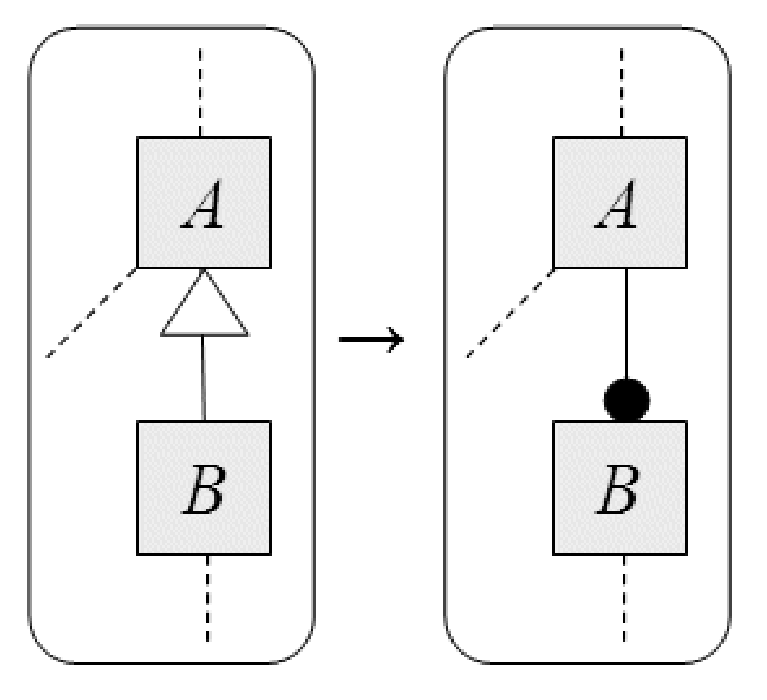
\includegraphics{images/bad-smell1.eps}}
\end{center}
\end{figure}

% template matching
Refactoring designers can apply general FM refactorings based on template matching. 
% templates
Each {\em general refactoring} consists of two {\em templates} (patterns) of FMs, on the left-hand (LHS) and right-hand (RHS) sides.
% quando podemos aplicar o refatoramento
A refactoring can be applied whenever the FM matches the template. A matching is an assignment of all meta-features occurring in the LHS template to concrete values.
% o que n�o e mostrado e igual nos dois modelos
Any element omitted by the templates remains unchanged, thus refactoring templates only show differences between FMs. 
% linhas pontilhadas
Moreover, a dashed line on top of a feature indicates that this feature may have a parent feature. A dashed line below a feature indicates that this feature may have additional subfeatures.

% o outro refactoring
A similar refactoring that converts an \emph{or} relation to a mandatory relation can be proposed. 
% corretude
Both refactorings and the following one can be shown correct using a encoding of FMs~\cite{Gheyi:2006aa} in Alloy~\cite{Jakson:2006aa} or using a Prototype Verification System (PVS)~\cite{Owre:2009aa} theory~\cite{Gheyi:2006aa-2}.

\subsection{Constraint imposing the selection of an alternative}

% 1. intuicao
Sometimes a constraint in the model may impose that a child of an alternative relation must always be selected. This bad smell occurs when a global constraint obligates the selection of an \emph{Alternative Feature} or \emph{Or Feature}.
% 2. porque � um problema?
\Fix{Leopoldo: sera que isto eh um problema quando nao eh uma feature
mandatoria que esta impondo a selecao de uma feature alternativa/or?} Since a child must always be selected, the other children of this relationship can never be selected. Detecting this kind of bad smell might reveal constraints that are inconsistent with the feature model relationships.

% 3. explicar em um exemplo toy
For instance, suppose that we add the constraint $B \Rightarrow D'$ in the feature model of Figure~\ref{fig:fm01}. Since B is a mandatory feature of A, it must be selected. From this fact and the previous constraint added, feature D' must be selected.  Therefore, only D' will be a valid option to the alternative feature D. The feature D'' can never be selected.
% conclusao
This may reveal a symptom of a bad design.
% 4. exemplo real

% 5. refatoramento
Refactoring~\ref{ref:ref2} removes this bad smell by excluding the constraint.

\begin{figure}[ht]
\begin{refine}{\ensuremath{\langle}change alternative constraint\ensuremath{\rangle}}
\label{ref:ref2}
\end{refine}
\begin{center}
\leavevmode
\scalebox{0.4}{
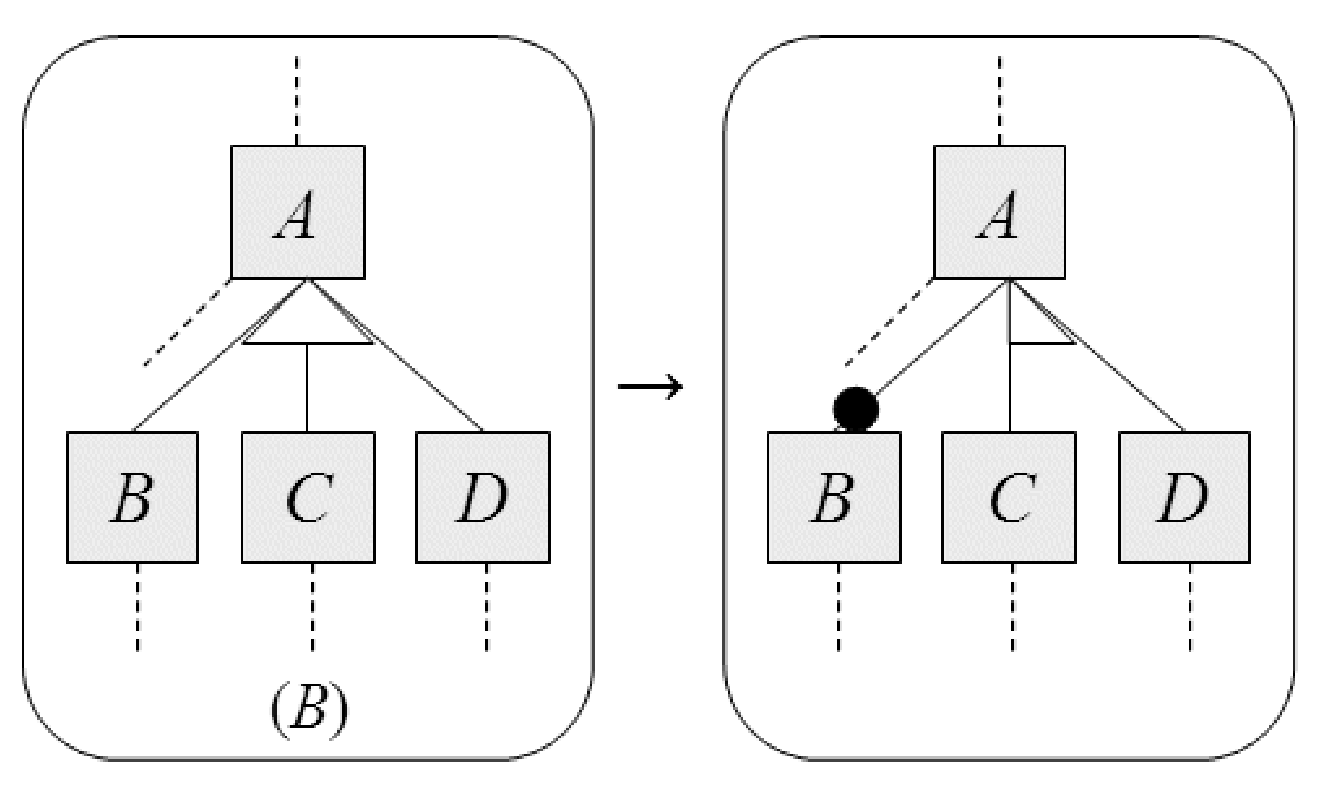
\includegraphics{images/bad-smell2.eps}}
\end{center}
\end{figure}

% refatoramento similar
A similar refactoring can be proposed for an \emph{Or} relationship.
% lei util
In this bad smell and in the following ones, which involve constraints (formulae), we may use Refactoring~\ref{ref:add-formula} in order to prepare the FM to match, for instance, Refactoring~\ref{ref:ref2} template. 
% explicando variavel
The \emph{fs} variable denotes a set of features.
% voltando ao exemplo
In the Figure~\ref{fig:fm01} feature model example, Refactoring~\ref{ref:add-formula} is used to deduce the constraint \emph{D'}. After that, we can apply Refactoring~\ref{ref:ref2}.

\begin{figure}[ht]
\begin{refine}{\ensuremath{\langle}add deducible formula\ensuremath{\rangle}}
\label{ref:add-formula}
\end{refine}
\begin{center}
\leavevmode
\scalebox{0.4}{
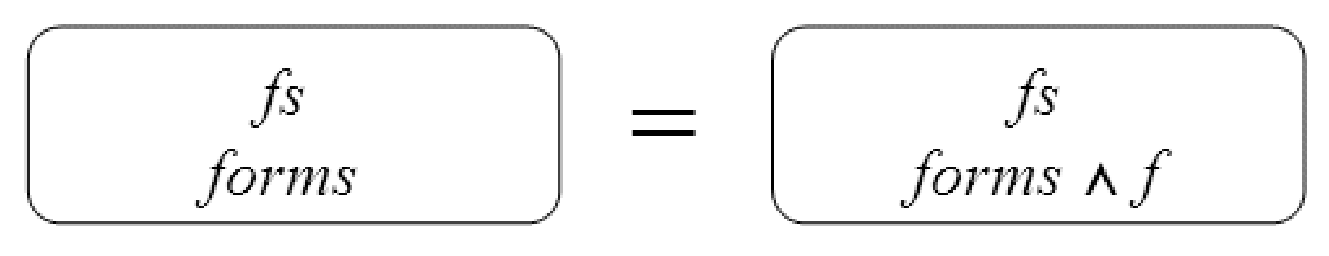
\includegraphics{images/add-formula.eps}}
\end{center}
\noindent ($\leftrightarrow$) \emph{f} can be deduced from \emph{forms} and \emph{fs}. \\
\end{figure}

\subsection{Constraint changing the semantics of a relationship}

% 1. intuicao
Sometimes a feature model may have a constraint making the semantics of a relationship more restrictive. 
% 2. porque � um problema?
This may waste time of domain analysts when understanding the model. It is better to change the relationship. It is easier to understand a model if we include most constraints in the graphical notation.
% 3. explicar em um exemplo toy
One example of this bad smell is present in the feature model of Figure~\ref{fig:fm01}.
As we explained in Section~\ref{sec:intro}, in the presence of the global constraint $B \Rightarrow D$, the optional relationship between the features A and D is changed to mandatory. Detecting this kind of bad smell reveals either an improper constraint or an inadequate feature model relationship.
% 4. exemplo real

% 5. refatoramento
This bad smell can be removed by applying Refactoring~\ref{ref:ref3}, which changes from the optional relationship to the mandatory relationship.

\begin{figure}[ht]
\begin{refine}{\ensuremath{\langle}replace optional to mandatory\ensuremath{\rangle}}
\label{ref:ref3}
\end{refine}
\begin{center}
\leavevmode
\scalebox{0.4}{
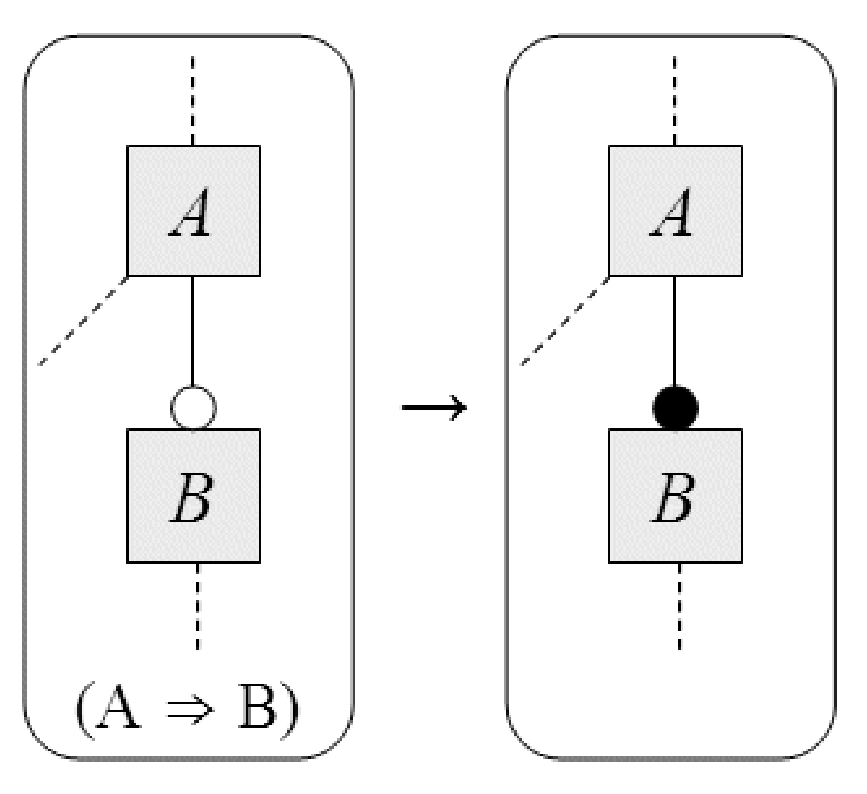
\includegraphics{images/bad-smell3.eps}}
\end{center}
\end{figure}

The same bad smell can appear between other relationships. For example, sometimes we can convert an \emph{Or} relationship to an \emph{Alternative} relationship. A number of refactorings can be useful for removing them~\cite{Gheyi:2009aa}.

\subsection{Redundant constraints}

% 1. intuicao
It is useful to add redundant constraints in order to make the model easier to understand. A redundant constraint does not narrow the number of instances (configurations) of a feature model --- so, it does not define any additional restriction to the feature model. The number of valid configurations is the same.
% 2. porque � um problema?
However, sometimes when we add a number of redundant constraints, it may be difficult for domain analysts to understand the entire model. They may waste time reading some constraints that does not add value to the model. So, in these situations, it may be better to remove them.

% 3. explicar em um exemplo toy
For example, suppose that one defines a constraint $C \Rightarrow B$ in the feature model of Figure~\ref{fig:fm01}, instead of writing a proper constraint. Note that such a constraint is redundant, since feature B must be present in any valid configuration of this feature model. 
% conclusao
Therefore, detecting this kind of bad smell might reveal a constraint that was not well specified. 
% 4. exemplo real
% 5. refatoramento
This bad smell can be removed by applying Refactoring~\ref{ref:add-formula} from right to left.

\subsection{Dead features}

% 1. intuicao
This bad smell occurs when a feature, due to a global constraint, could never be selected in the valid instances of a feature model~\cite{Trindad:2006aa}. It may happen because of the number of constraints in the model that may make the model difficult to understand, hence suitable for introducing errors.
% 2. porque � um problema?
This may be a symptom of a bad design. 

% 3. explicar em um exemplo toy
For instance, if the constraint $B \Rightarrow \neg C $ is added to the feature model of Figure~\ref{fig:fm01}, the feature C becomes a dead feature. It will never be present in any configuration of the feature model. 
% conclusao
If a feature is dead, it may be useless to the model and should be removed from it, or it may reveal a problem in the model (overconstrained) and we should remove some constraints.

% 4. exemplo real
% 5. refatoramento
Two refactorings can be used to remove this bad smell. Refactoring~\ref{ref:remove-formula} can be used to remove some constraints in the overconstrained model. 

\begin{figure}[ht]
\begin{refine}{\ensuremath{\langle}remove formula\ensuremath{\rangle}}
\label{ref:remove-formula}
\end{refine}
\begin{center}
\leavevmode
\scalebox{0.4}{
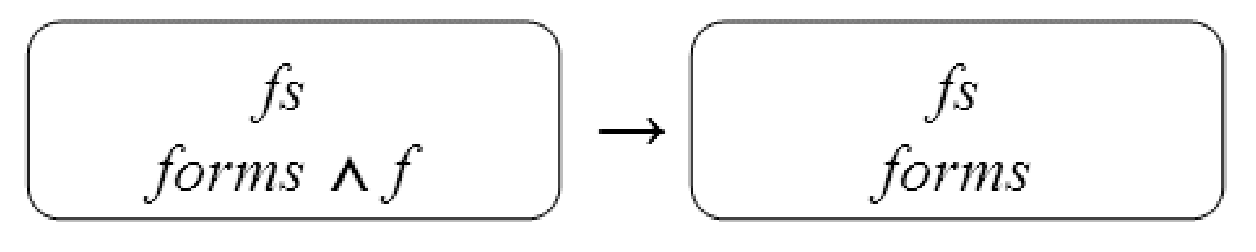
\includegraphics{images/remove-formula.eps}}
\end{center}
\end{figure}

In case the feature must be removed, we can apply Refactoring~\ref{ref:remove-feature}. We remove it from the model, and replace its occurrence in all constraints by \emph{false}.

\begin{figure}[ht]
\begin{refine}{\ensuremath{\langle}remove dead feature\ensuremath{\rangle}}
\label{ref:remove-feature}
\end{refine}
\begin{center}
\leavevmode
\scalebox{0.4}{
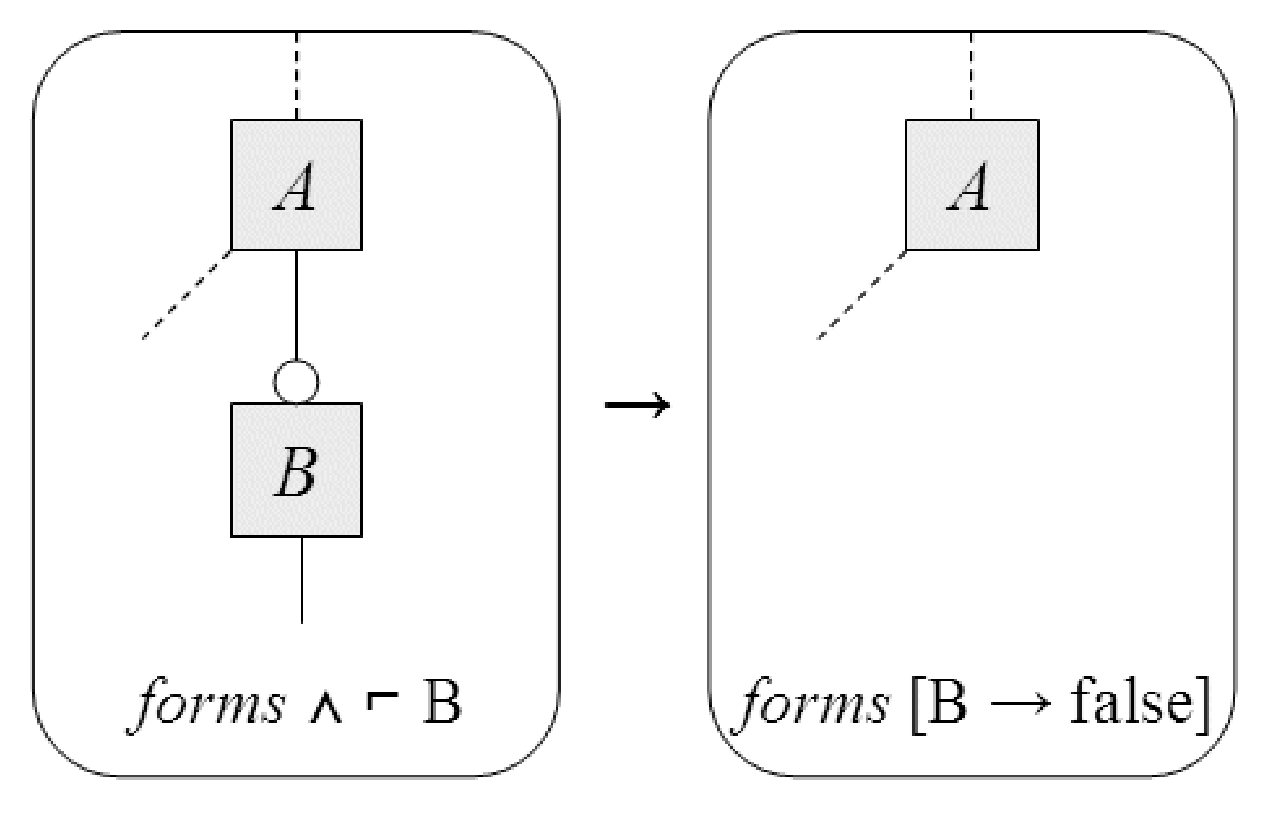
\includegraphics{images/remove-feature.eps}}
\end{center}
\end{figure}

\subsection{Inconsistent Model}

% 1. intuicao
This bad smell occurs when a feature model does not have any valid
configuration due to contradicting constraints. It may happen when
overconstraining the model, making it difficult to understand, hence, suitable
for introducing errors.
% 2. porque � um problema?
In general, this may be a symptom of a bad design and an error. 

% 3. explicar em um exemplo toy
For instance, if the constraint $C \Rightarrow \neg D $ is added to the feature
model of Figure~\ref{fig:fm01}, the model becomes inconsistent. The feature D
must always be selected.
% conclusao
If a model does not have a valid configuration, it may reveal an error in the
model design. In general, it is useless to have an inconsistent model.

% 4. exemplo real
% 5. refatoramento
In order to remove the contradiction, we first use a tool, such as proposed by Benavides~\cite{Trinidad:2008aa-2}, which extracts the minimum set of constraints that make the model inconsistent. After debugging the model, the domain analyst should check which set of constraints must be removed. Then, we can apply Refactoring~\ref{ref:remove-formula} to remove them from the model.


